%%% LaTeX Template: Article/Thesis/etc. with colored headings and special fonts
%%%
%%% Source: http://www.howtotex.com/
%%% Feel free to distribute this template, but please keep to referal to http://www.howtotex.com/ here.
%%% February 2011
%%%
%%% Modified January 2016 by CDM

%%%  Preamble
\documentclass[11pt,letterpaper]{article}
\usepackage[margin=1.0in]{geometry}
\usepackage[T1]{fontenc}
\usepackage[bitstream-charter]{mathdesign}
\usepackage[latin1]{inputenc}					
\usepackage{amsmath}						
\usepackage{xcolor}
\usepackage{cite}
\usepackage{hyphenat}
\usepackage{graphicx}
\usepackage{float}
\usepackage{subfigure}
\usepackage{sectsty}
\usepackage[compact]{titlesec} 
\usepackage[tablegrid]{vhistory}
\usepackage{pbox}
\allsectionsfont{\color{accentcolor}\scshape\selectfont}

%%% Definitions
\definecolor{accentcolor}{rgb}{0.0,0.0,0.5} 
\newcommand{\teamname}{LJCJ}
\newcommand{\productname}{UR20}
\newcommand{\coursename}{CSE 4316: Senior Design I}
\newcommand{\semester}{Fall 2024}
\newcommand{\docname}{Architectural Design Specification}
\newcommand{\department}{Department of Computer Science \& Engineering}
\newcommand{\university}{The University of Texas at Arlington}
\newcommand{\authors}{Luis Contreras \\ Joushua Dominguez \\ Christopher Gonzalez \\ Jasper Gustafson}

%%% Headers and footers
\usepackage{fancyhdr}
	\pagestyle{fancy}						% Enabling the custom headers/footers
\usepackage{lastpage}	
	% Header (empty)
	\lhead{}
	\chead{}
	\rhead{}
	% Footer
	\lfoot{\footnotesize \teamname \ - \semester}
	\cfoot{}
	\rfoot{\footnotesize page \thepage\ of \pageref{LastPage}}	% "Page 1 of 2"
	\renewcommand{\headrulewidth}{0.0pt}
	\renewcommand{\footrulewidth}{0.4pt}

%%% Change the abstract environment
\usepackage[runin]{abstract}			% runin option for a run-in title
%\setlength\absleftindent{30pt}			% left margin
%\setlength\absrightindent{30pt}		% right margin
\abslabeldelim{\quad}	
\setlength{\abstitleskip}{-10pt}
\renewcommand{\abstractname}{}
\renewcommand{\abstracttextfont}{\color{accentcolor} \small \slshape}	% slanted text

%%% Start of the document
\begin{document}

%%% Cover sheet
{\centering \huge \color{accentcolor} \sc \textbf{\department \\ \university} \par}
\vspace{1 in}
{\centering \huge \color{accentcolor} \sc \textbf{\docname \\ \coursename \\ \semester} \par}
\vspace{0.5 in}
\begin{figure}[h!]
	\centering
   	
\includegraphics[width=0.60\textwidth]{images/LJCJ}
\end{figure}
\vspace{0.5 in}
{\centering \huge \color{accentcolor} \sc \textbf{\teamname \\ \productname} \par}
\vspace{0.5 in}
{\centering \large \sc \textbf{\authors} \par}
\newpage


%\vspace{1 in}
%\centerline{January 13th, 2012}
%\newpage

%%% Revision History
\begin{versionhistory}
  	\vhEntry{0.1}{11.11.2024}{LC, JD, CG, JG}{Document creation}

\end{versionhistory}
\newpage

%%% Table of contents
\setcounter{tocdepth}{2}
\tableofcontents
\newpage

%%% List of figures and tables (optional)
\listoffigures
\listoftables
\newpage

%%% Document sections
\section{Introduction}
Your introduction should provide a brief overview of the product concept and a reference to the requirement specification and architectural design documents in 1 or 2 paragraphs. The purpose is to provide the reader with the location of relevant background material that lead to the design details presented in this document.

\newpage
\section{System Overview}
The overall structure of the software system is designed to seamlessly support the palletizing tasks of the UR20 robot arm system. This layered design enables modular functionality, enhancing system adapability and ensuring each layer performs a unique function while simultaneously providing crucial information to the main PLC layer which manages data distribution. As the central interface, the PLC efficiently processes the flow of sata from each subsystem layer, allowing for smooth system integration and effective coordination across all layers. This architecture promotes reliable, dynamic operation, optimizing the UR20's performance in real-time palletizing tasks.
\begin{figure}[h!]
	\centering
 	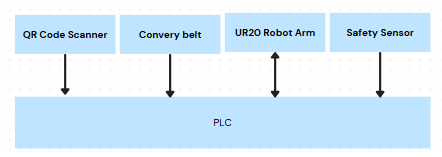
\includegraphics[width=0.60\textwidth]{images/layers}
 \caption{UR20 Architectural design diagram}
\end{figure}

\subsection{Layer 1: PLC Description}
The PLC will process most of the data through its peripherals, as seen in Figure 1. It is the primary interface between the different layers of the project. The built-in PLC will be configured with URScript, a Python-based scripting language in which vital functions will reside, such as the input function, the box offset algorithm, and finally, a position algorithm. The data flow will start with the input given by the QR code scanner or the safety sensor, and the input functions will follow these two data paths. First being, an input given by the QR code scanner will pass through the input function, which will then call the box offset algorithm to determine where the box is in 3D space given the location info from the QR code, which will go to the position algorithm which will determine the motion necessary for the UR20 to satisfy this request. The safety algorithm will give the second path, which will trigger the input function and call the position algorithm to safely slow down the speed at which the UR20 is palletizing to create a safe work area for a cooperative application.

\subsection{Layer 2: Safety Sensor}
The Safety Sensor will determine if a human is in the area of the UR20 arm. If so, it will reduce the speed of the UR20 in order to create a safe work environment. This will be achieved with the use of a camera that will process the data in real-time with the use of computer vision, which will send a signal to the PLC which in turn will send a signal to the UR20 movement subsystem in order to maintain a safe speed for collaborative work.

\subsection{Layer 3: UR20 Robot Arm}
UR20 Arm consists of a vacuum gripper, the gripper controller, and the movement of the arm. The arm is the physical output of the software that resides in the PLC layer. Additionally, it contains a gripper grab/release controller (the controller for the air compressor), which will be turned on or off when needed to hold or drop a box. The commands given by the PLC will determine the position and orientation needed for the UR20 to place the box correctly.

\subsection{Layer 4: QR Code Scanner}
Implementing QR code technology will enhance the automation and accuracy of arranging boxes on a pallet. When a box arrives on the conveyor belt, a QR code scanner positioned above the belt reads the QR code on the box. This QR code contains data such as box size, weight, and any other relevant handling instructions. Once scanned, the data is immediately sent to a Programmable Logic Controller (PLC) on a Universal Robots UR20 robotic arm system, which is responsible for arranging the boxes on the pallet.

\subsection{Layer 5: Conveyor Belt}
The conveyor belt system moves over pulleys driven by a motor. As the motor rotates, it propels the belt forward, allowing items placed on the belt to be conveyed along its length. The belt's speed can be adjusted to control the pace of movement. However, for this implementation, it will have two states: on or off. At the end of the conveyor belt, there will be a guide to reorient the boxes and a bracket in which the QR code scanner will be placed.
\newpage
\section{Subsystem Definitions \& Data Flow}

\begin{itemize}
    \item \textbf{Conveyor Belt Layer}
    \begin{itemize}
        \item ON/OFF Controller
    \end{itemize}

    \item \textbf{Safety Sensor Layer}
    \begin{itemize}
        \item Computer Vision
        \item UR20 Arm Speed Controller
    \end{itemize}

    \item \textbf{QR Layer}
    \begin{itemize}
        \item Scanner
        \item PLC Interface
    \end{itemize}

    \item \textbf{UR20 Robot Arm Layer}
    \begin{itemize}
        \item Vacuum Gripper
        \item Grab Release Control
        \item Movement
    \end{itemize}

    \item \textbf{PLC Layer}
    \begin{itemize}
        \item Input Function
        \item Box Offset Algorithm
        \item Position Algorithm
    \end{itemize}
\end{itemize}
\begin{figure}[h!]
	\centering
 	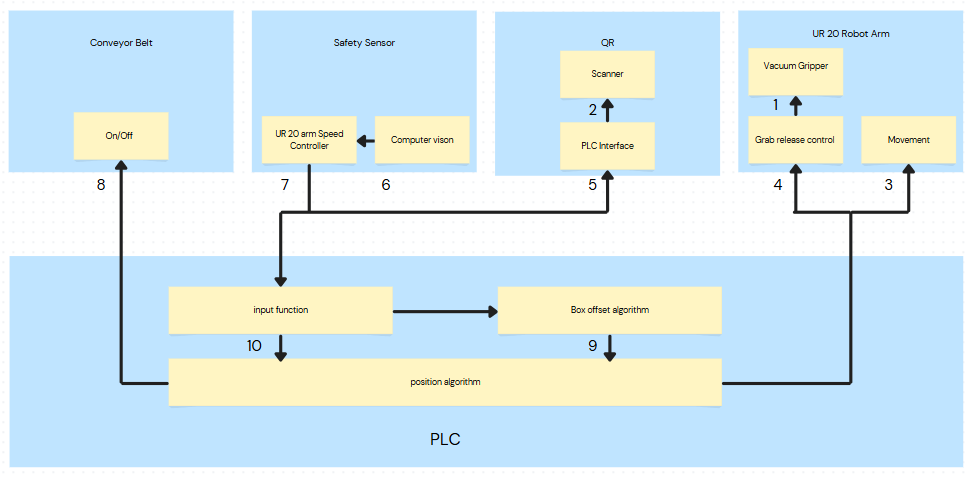
\includegraphics[width=\textwidth]{images/data_flow}
 \caption{UR20 Data flow diagram}
\end{figure}
\newpage
\section{PLC Layer Subsystems}
The UR20 has a system to practically create a single interface between the robot and PLC, in order to enhance the capabilities and functions of the cobot

\begin{figure}[h!]
	\centering
 	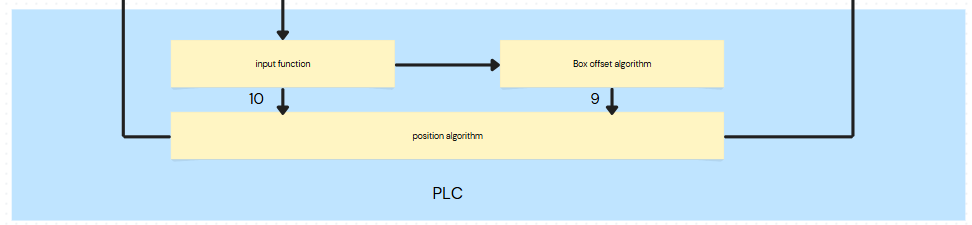
\includegraphics[width=0.60\textwidth]{images/Plc}
 \caption{PLC }
\end{figure}

\subsection{Input function}
The input function would be the readings of the environment knowing the positions of the pallet and reading the incoming box QR code 

\subsubsection{Assumptions}
Assumptions for the input function is that the boxes would have a visible QR code for sensor to read thus orientation of the box to be predefined. 

\subsubsection{Responsibilities}
The responsibitilies of the input fuction is soley to gather data that the PLC placement algorithm will use to preform its next action. such as the QR of the next box, the current state of the pallet, the location of any other nearby objects or people for safety concerns.

\subsubsection{Subsystem Interfaces}

\begin {table}[H]
\caption {Input fuction interfaces} 
\begin{center}
    \begin{tabular}{ | p{1cm} | p{6cm} | p{3cm} | p{3cm} |}
    \hline
    ID & Description & Inputs & Outputs \\ \hline
    \#01 & movement readings  & \pbox{3cm}{ destination\\position \\ speeds \\ safety sensor\\griper power} & \pbox{3cm}{formated data for PLC algorithm}  \\ \hline
    \#02 & box detection   & \pbox{3cm}{ QR reading\\position \\ speeds \\ safety sensor\\ griper power} & \pbox{3cm}{formated data for box offset algorithm }  \\ \hline
    
    \end{tabular}
\end{center}
\end{table}

\subsection{Box offset algorithm}
The box offset algorithm will be used to scan and determine the placement of the box 

\subsubsection{Assumptions}
QR codes will be used as a predefined locations for each bot and expected specfic order

\subsubsection{Responsibilities}
The responsibitilies of the placement function will be used to determine location of the box in the x,y,z dimentional plane and send it to the placement algorithm

\subsubsection{Subsystem Interfaces}


\begin {table}[H]
\caption {Box Offset algorithm interfaces} 
\begin{center}
    \begin{tabular}{ | p{1cm} | p{6cm} | p{3cm} | p{3cm} |}
    \hline
    ID & Description & Inputs & Outputs \\ \hline
    \#03 & movement  & \pbox{3cm}{QR reading\\position \\ speeds \\ safety sensor\\ griper power} & \pbox{3cm}{formated data for PLC algorithm }  \\ \hline
    
    \end{tabular}
\end{center}
\end{table}

\subsection{Placement algorithm }
The placement algorim is the central control of operations will tell the subsystems of the UR20 what actions to take given the output of the input function

\subsubsection{Assumptions}
The placement algorithm assumes that the gripper will have fixed strenght while moving a box and will be able to place without droping it. It expects belt and pallet location to be fixed and box orientation constant

\subsubsection{Responsibilities}
The responsibitilies of the placement function will be prefom send the appropriate values to the motors, in order to move arm to pick up the box then place it on pallet, and vacuum gripper to pick up and release the boxes. The algorithm will also be checking for safety based on the sensor to scan for people and stop or slow down movement.

\subsubsection{Subsystem Interfaces}


\begin {table}[H]
\caption {Placement algorithm interfaces} 
\begin{center}
    \begin{tabular}{ | p{1cm} | p{6cm} | p{3cm} | p{3cm} |}
    \hline
    ID & Description & Inputs & Outputs \\ \hline
    \#04 & movement  & \pbox{3cm}{QR reading\\destination\\ position \\ speeds \\ safety reading} & \pbox{3cm}{adjusted motor spreeds}  \\ \hline
    \#05 & gripper power  & \pbox{3cm}{destination\\postion} & \pbox{3cm}{ON/OFF}  \\ \hline
    
    \end{tabular}
\end{center}
\end{table}



\newpage
\section{Safety Sensor Layer Subsystems}
In this section, the layer is described in some detail in terms of its specific subsystems. Describe each of the layers and its subsystems in a separate chapter/major subsection of this document. The content of each subsystem description should be similar. Include in this section any special considerations and/or trade-offs considered for the approach you have chosen.



\begin{figure}[h!]
	\centering
 	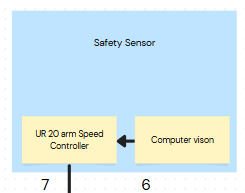
\includegraphics[width=0.60\textwidth]{images/safety_sens}
 \caption{Example subsystem description diagram}
\end{figure}

\subsection{UR 20 arm speed controller}
The controller will determine whether there is a person within the working vicinity of the UR20 robot and signal the PLC to adjust for the case
\subsubsection{Assumptions}
The UR20 should have collision detection and should stop at impact

\subsubsection{Responsibilities}
To signal the PLC the presence of a person near the robot using a computer vision algorithm

\subsubsection{Subsystem Interfaces}


\begin {table}[H]
\caption {Speed Controller Subsystem Interface} 
\begin{center}
    \begin{tabular}{ | p{1cm} | p{6cm} | p{3cm} | p{3cm} |}
    \hline
    ID & Description & Inputs & Outputs \\ \hline
    \#06 & send signal & \pbox{3cm}{presence detection} & \pbox{3cm}{presence signal}  \\ \hline
    \end{tabular}
\end{center}
\end{table}

\subsection{Computer vision algorithm}
A computer vision algorithm to scan for the presence of a person being near the UR20 robot
\subsubsection{Assumptions}
assume that the camera has a good point of view as to beable to see all around the robot 

\subsubsection{Responsibilities}
Inform controller of detected pressence near the UR20 

\subsubsection{Subsystem Interfaces}


\begin {table}[H]
\caption {Computer Vision Subsystem Interface} 
\begin{center}
    \begin{tabular}{ | p{1cm} | p{6cm} | p{3cm} | p{3cm} |}
    \hline
    ID & Description & Inputs & Outputs \\ \hline
    \#07 & presence detection & \pbox{3cm}{camera reading} & \pbox{3cm}{presence detection}  \\ \hline
    \end{tabular}
\end{center}
\end{table}


\newpage
\section{UR 20 Arm Layer Subsystems}
The UR20 arm is a layer controlled by the PLC used exclusively for manipulation. It is a collaborative robot arm that will be used to grab the boxes and position them upon the pallet. It has three subsystems: the movement interface, the vacuum gripper, and the vacuum gripper controller.

\begin{figure}[h!]
	\centering
 	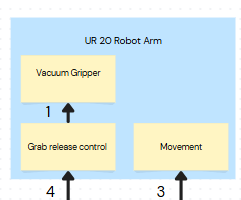
\includegraphics[width=0.60\textwidth]{images/UR20_ARM}
 \caption{UR20 Robot Arm Layer}
\end{figure}

\subsection{Movement}
This subsystem of the UR20 arm is technically an interface within the PLC, but as the PLC and UR20 are married so closely together, and this is more closely related to the arm itself, it is listed as a subsystem of the arm. The interface will allow easy control of the arm's movements. Its input is data from the PLC's decision making algorithm and its output is to directly control the robot's movements.

\subsubsection{Assumptions}
The assumption being made is that the UR20 arm is going to exclusively be a tool of the PLC, and thus will only interface with the PLC. The movement interface may even be built into the PLC for this robot, as it seems to be with some other UR cobots, but as of right now it is being assumed that a control system will have to be programmed for it on the PLC.

\subsubsection{Responsibilities}
The responsibility of the movement subsystem is to translate the box location, current arm location, and current desired speed into a coherent set of movements for the UR20 arm. These factors will be combined to create a set of movements and movement speed that will move the arm to the desired location. This must account for the position of the QR scanner when deciding where to place the arm.

\subsubsection{Movement Subsystem Interfaces}
Each of the inputs and outputs for the subsystem are defined here.

\begin {table}[H]
\caption {Movement interface} 
\begin{center}
    \begin{tabular}{ | p{1cm} | p{6cm} | p{3cm} | p{3cm} |}
    \hline
    ID & Description & Inputs & Outputs \\ \hline
    \#08 & Change in X,Y,Z Coordinates & \pbox{3cm}{X \\ Y \\ Z} & \pbox{3cm}{NO OUTPUT}  \\ \hline
    \#09 & Movement Speed & \pbox{3cm}{Speed} & \pbox{3cm}{NO OUTPUT}  \\ \hline
    \#10 & Rotation Angles & \pbox{3cm}{Perpendicular \\ Longitudinal} & \pbox{3cm}{NO OUTPUT}  \\ \hline
    \end{tabular}
\end{center}
\end{table}

\subsection{Vacuum Gripper}
    The vacuum gripper is physical hardware and its software inputs and outputs are covered in the Vacuum Gripper Controller subsystem. The vacuum gripper is connected to a vacuum generator that will be adjusted to provide a static amount of force capable of picking the boxes and not dropping them until the controller determines that it should do so.

\subsubsection{Assumptions}
The vacuum gripper will be a hardware-only system with a constant vacuum that can be blocked in order to drop a box. It will interface exclusively with the vacuum gripper controller and have no outputs.

\subsubsection{Responsibilities}
The responsibility of the vacuum gripper is to securely hold and transport boxes. It will be able to drop the boxes on command and in the process it will shift the boxes as little as possible in order to produce the expected placement.

\subsubsection{Movement Subsystem Interfaces}
Each of the inputs and outputs for the subsystem are defined here.

\begin {table}[H]
\caption {Movement interface} 
\begin{center}
    \begin{tabular}{ | p{1cm} | p{6cm} | p{3cm} | p{3cm} |}
    \hline
    ID & Description & Inputs & Outputs \\ \hline
    \#11 & Vacuum Control Signal & \pbox{3cm}{ONOFF} & \pbox{3cm}{NO OUTPUT}  \\ \hline
    \end{tabular}
\end{center}
\end{table}

\subsection{Vacuum Gripper Controller}
The vacuum gripper controller is the software interface between the PLC and the vacuum gripper. It signals the vacuum hardware to kill the vacuum and drop the box being held. 

\subsubsection{Assumptions}
The vacuum gripper controller will be on at all times EXCEPT when it is told that a box needs to be dropped. 

\subsubsection{Responsibilities}
The vacuum gripper controller must turn off the vacuum long enough for the cobot to move away, which should occur soon after. If it turns on again too soon, the box will be pulled out of the desired position. 

\subsubsection{Movement Subsystem Interfaces}
Each of the inputs and outputs for the subsystem are defined here.

\begin {table}[H]
\caption {Movement interface} 
\begin{center}
    \begin{tabular}{ | p{1cm} | p{6cm} | p{3cm} | p{3cm} |}
    \hline
    ID & Description & Inputs & Outputs \\ \hline
    \#12 & Drop Signal & \pbox{3cm}{Trigger} & \pbox{3cm}{ONOFF}  \\ \hline
    \#13 & Current Speed & \pbox{3cm}{Speed} & \pbox{3cm}{NO OUTPUT}  \\ \hline
    \end{tabular}
\end{center}
\end{table}


\newpage
\section{QR Layer Subsystems}
The QR Layer consists of two primary subsytems: the Scanner and PLC interface. This layer is responsible for scanning the QR codes on each box, retrieving the relevant data (box size, weight, center position) and transmitting the data to the PLC for further processing.

\begin{figure}[h!]
	\centering
 	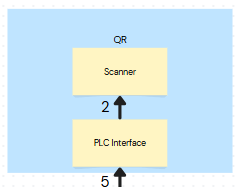
\includegraphics[width=0.60\textwidth]{images/Qr}
 \caption{Example subsystem description diagram}
\end{figure}


\subsection{Scanner}
The scanner subsystem is responsible for reading the QR codes on boxes as they enter the field of view of the camera. The QR codes will be positioned in the center of each box strategicall so as to be able to extract the data related to the box's dimesinons and position. The data is then forwarded to the PLC interface for processing byb the PLC.
\subsubsection{Assumptions}
The assumption is that all boxes on the conveyor belt will have QR codes correctly positioned and free from any obstructions. The scanner will only scan one box at a time and have ample time process the information, as well as re-process if there are any miss readings or missing information from the QR code.

\subsubsection{Responsibilities}
The sole responsibilty of the scanner is to read the QR codes on the boxes, parsing essential box dat into a format that is compatible with the PLC interface. Data is only transmitted when a successful scan is achieved.

\subsubsection{Subsystem Interfaces}

\begin {table}[H]
\caption {Scanner Subsystem interface} 
\begin{center}
    \begin{tabular}{ | p{1cm} | p{6cm} | p{3cm} | p{3cm} |}
    \hline
    ID & Description & Inputs & Outputs \\ \hline
    \#14 & QR code interface & \pbox{3cm}{QR code } & \pbox{3cm}{Parsed box data}  \\ \hline
    \end{tabular}
\end{center}
\end{table}

\subsection{PLC Interface Subsystem}
The PLC interface subsystem acts as a bridge between the scanner and the PLC. After receiving the parsed box data from the scanner, it formats and transmits this information to the PLC's input function. This subsystem esnures that the data is correctly structed for further processing in the PLC, allowing the system to execute appropriate palletizing commands based on the box dimesnions.
\subsubsection{Assumptions}
The data from the scanner is received in a standardized format, requiring minimal processing before it reaches the PLC. The PLC interface does not need to handle multiple data streams simultaneously, as each box is processed sequentially.

\subsubsection{Responsibilities}
The responsibility of the PLC interface subsystem is to format the data as required by the PLC's input function, and esnure smooth communication between the scanner and PLC systems.

\subsubsection{Subsystem Interfaces}

\begin {table}[H]
\caption {Scanner Subsystem interface} 
\begin{center}
    \begin{tabular}{ | p{1cm} | p{6cm} | p{3cm} | p{3cm} |}
    \hline
    ID & Description & Inputs & Outputs \\ \hline
    \#15 & Data transfer for PLC & \pbox{3cm}{Parsed box data from Scanner} & \pbox{3cm}{Formatted data for PLC Input function}  \\ \hline
    \end{tabular}
\end{center}
\end{table}



\newpage
\section{Conveyor Belt Layer Subsystems}
The conveyor belt layer is managed by the PLC and is solely responsible for controlling the conveyor belts movement. This layer has one subsystem: The ON/OFF controller, which recieves signals from the PLC to start or stop the conveyor belt based on when the UR20 robot arm is ready to receive another box. The control of the conveyor belt is simplified to an ON/OFF mechanism, rather than dyanmically adjusting speed based on palletizing rate.

\begin{figure}[h!]
	\centering
 	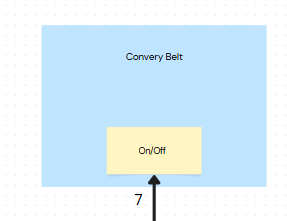
\includegraphics[width=0.60\textwidth]{images/convery_belt}
 \caption{Conveyor Belt Power Controller}
\end{figure}
\subsection{Power Controller Subsystem}
The power contoller subsystem in the conveyor belt layer is responsible for controlling the state of the conveyor belt. The subsystem receives a command from the PLC to switch the belt "ON" when the robot is prepared to recieve a new box and "OFF" once the box has been processed, ensuring smooth and controlled movement of boxes.
\subsubsection{Assumptions}
The assumption of a required automatic speed control is not required. The belts state change is assumed to be sufficient for the palletizing application, without the need to detect the exact positions of boxes on the belt. Only ensuring that the boxed move in a controlled manner when ready.

\subsubsection{Responsibilities}

The power controllers main responsibility is to maintain the stability of the conveyor, preventing any from advancing too far or falling off during the palletizing process. By managing the conveyor's ON/OFF state, it ensures that boxes are presented to the robot in a timely and safe manner. 

\subsubsection{Subsystem Interfaces}
The ON/OFF signal from the PLC serves as the sole input for the power controller. When the PLC sends an "ON" signal, the conveyor belt starts moving and will stop movement when the "OFF" signal is received. 

\begin {table}[H]
\caption {Controller Interface} 
\begin{center}
    \begin{tabular}{ | p{1cm} | p{6cm} | p{3cm} | p{3cm} |}
    \hline
    ID & Description & Inputs & Outputs \\ \hline
    \#16 & Power Controller signal & \pbox{3cm}{ ON/OFF } & \pbox{3cm}{NO OUTPUT}  \\ \hline
    \end{tabular}
\end{center}
\end{table}



\newpage


%%% References
\bibliographystyle{plain}
\bibliographystyle{reference/IEEEtran_custom}
\bibliography{reference/refs}{}

\end{document}